\documentclass[journal]{IEEEtran}
\usepackage[a5paper, margin=10mm, onecolumn]{geometry}
\usepackage[cmex10]{amsmath}
\usepackage{amssymb,amsfonts,amsthm}
\usepackage{gvv-book}
\usepackage{gvv}
\usepackage{hyperref}

\begin{document}

\title{1.5.13}
\author{EE25BTECH11025 - Ganachari Vishwambhar}
\maketitle

\textbf{Question}:\newline
Find the ratio in which the $Y$ axis divides the line segment joining the points $\vec{A}\brak{-1,-4}$ and $\vec{B}\brak{5,-6}$. Also find the coordinates of the point of intersection.\\
\textbf{Solution: }\\

Given points are:
\begin{align}
\vec{A}=\myvec{-1\\-4}
\vec{B}=\myvec{5\\-6}
\end{align}

Let the line segment joining $\vec{A}$ and $\vec{B}$ intersect the X=0 at point $\vec{C}$. Let the ratio in which the X=0 divide the line segment $\vec{B}-\vec{A}$ be $m:1$:
\begin{align}
\vec{C}=\myvec{0\\a}
\end{align}

Points $\vec{A}$, $\vec{B}$ and $\vec{C}$ are collinear, so vectors $\vec{B}-\vec{A}$ and $\vec{C}-\vec{A}$ are parallel.\\
Collinearity leads to:
\begin{align}
    rank\brak{\vec{B}-\vec{A},\vec{C}-\vec{A}}
\end{align}
Matrix setup:
\begin{align}
    \myvec{-6&-5\\2&a+6}\\
    R_2 \rightarrow R_2 + \frac{1}{3}R_3\\
\end{align}
Echelon form:
\begin{align}
    \myvec{-6&-5\\0&a+\frac{13}{3}}
\end{align}
For rank = 1, the second row must be all zeroes:
\begin{align}
    a+\frac{13}{3}=0\\
    a=\brak{\frac{-13}{3}}
\end{align}

Thus the coordinates of point $\vec{C}$:
\begin{align}
    \vec{C}=\myvec{0\\\frac{-13}{3}}
\end{align}

Finding $m$ by projecting $\vec{C}-\vec{A}$ onto the direction of $\vec{B}-\vec{A}$:
\begin{align}
    m=\frac{\myvec{5 & \frac{-5}{3}}\myvec{1 \\ \frac{-1}{3}}}{\norm{\myvec{1 \\ \frac{-1}{3}}}^2}=5
\end{align}

Thus, the ratio in which the point $\vec{C}$ divides the line segment $\vec{B}-\vec{A}$ is \textbf{5:1}. \\

\begin{figure}[h!]
   \centering
   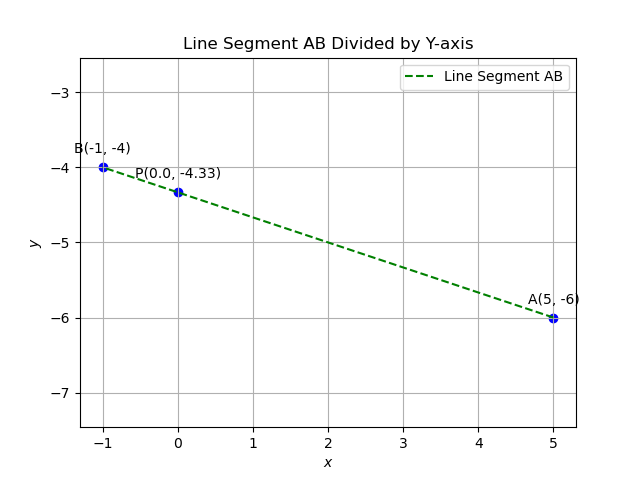
\includegraphics[width=0.7\linewidth]{figs/plot.png}
   \caption{Plot of line segment \textbf{B-A}}
   \label{}
\end{figure}
\end{document}  
